% The comment below tells Rubber to compile the .dot files.
%
% rubber: module graphics
% rubber: rules rules.ini

\documentclass[aspectratio=169]{beamer}

\usetheme{default}

\usefonttheme{structurebold}
\usepackage{helvet}
\usecolortheme{seagull}         % white on black

\usepackage[utf8]{inputenc}
\PassOptionsToPackage{hyphens}{url}\usepackage{hyperref,xspace,multicol}
\usepackage[absolute,overlay]{textpos}
\usepackage{tikz}
\usetikzlibrary{arrows,shapes,trees,shadows,positioning}
\usepackage{fancyvrb}           % for '\Verb'
\usepackage{xifthen}            % for '\isempty'

% Remember the position of every picture.
\tikzstyle{every picture}+=[remember picture]

\tikzset{onslide/.code args={<#1>#2}{%
  \only<#1>{\pgfkeysalso{#2}} % \pgfkeysalso doesn't change the path
}}

% Colors.
\definecolor{guixred1}{RGB}{226,0,38}  % red P
\definecolor{guixorange1}{RGB}{243,154,38}  % guixorange P
\definecolor{guixyellow}{RGB}{254,205,27}  % guixyellow P
\definecolor{guixred2}{RGB}{230,68,57}  % red S
\definecolor{guixred3}{RGB}{115,34,27}  % dark red
\definecolor{guixorange2}{RGB}{236,117,40}  % guixorange S
\definecolor{guixtaupe}{RGB}{134,113,127} % guixtaupe S
\definecolor{guixgrey}{RGB}{91,94,111} % guixgrey S
\definecolor{guixdarkgrey}{RGB}{46,47,55} % guixdarkgrey S
\definecolor{guixblue1}{RGB}{38,109,131} % guixblue S
\definecolor{guixblue2}{RGB}{10,50,80} % guixblue S
\definecolor{guixgreen1}{RGB}{133,146,66} % guixgreen S
\definecolor{guixgreen2}{RGB}{157,193,7} % guixgreen S

\setbeamerfont{title}{size=\huge}
\setbeamerfont{frametitle}{size=\huge}
\setbeamerfont{normal text}{size=\Large}

% White-on-black color theme.
\setbeamercolor{structure}{fg=guixorange1,bg=black}
\setbeamercolor{title}{fg=white,bg=black}
\setbeamercolor{date}{fg=guixorange1,bg=black}
\setbeamercolor{frametitle}{fg=white,bg=black}
\setbeamercolor{titlelike}{fg=white,bg=black}
\setbeamercolor{normal text}{fg=white,bg=black}
\setbeamercolor{alerted text}{fg=guixyellow,bg=black}
\setbeamercolor{section in toc}{fg=white,bg=black}
\setbeamercolor{section in toc shaded}{fg=white,bg=black}
\setbeamercolor{subsection in toc}{fg=guixorange1,bg=black}
\setbeamercolor{subsection in toc shaded}{fg=white,bg=black}
\setbeamercolor{subsubsection in toc}{fg=guixorange1,bg=black}
\setbeamercolor{subsubsection in toc shaded}{fg=white,bg=black}
\setbeamercolor{frametitle in toc}{fg=white,bg=black}
\setbeamercolor{local structure}{fg=guixorange1,bg=black}

\newcommand{\highlight}[1]{\alert{\textbf{#1}}}

\title{Controlling Software Environments with GNU~Guix}

\author{Ludovic Courtès}
\date{\small{Inria Bordeaux Sud-Ouest\\November 2016}}

\setbeamertemplate{navigation symbols}{} % remove the navigation bar

\AtBeginSection[]{
  \begin{frame}
    \frametitle{}
    \tableofcontents[currentsection]
  \end{frame} 
}


\newcommand{\screenshot}[2][width=\paperwidth]{
  \begin{frame}[plain]
    \begin{tikzpicture}[remember picture, overlay]
      \node [at=(current page.center), inner sep=0pt]
        {\includegraphics[{#1}]{#2}};
    \end{tikzpicture}
  \end{frame}
}


\begin{document}

\maketitle

\setbeamercolor{normal text}{bg=guixblue2}
\begin{frame}
  \Huge{\textbf{The difficulty of keeping software environments under
      control.}}
\end{frame}
\setbeamercolor{normal text}{fg=white,bg=black}

\begin{frame}[plain]
  \Huge{\#1. Upgrades are hard.}
\end{frame}

\setbeamercolor{normal text}{bg=white}
\screenshot[height=0.9\paperheight]{images/debian-upgrade-warning}
\screenshot{images/debian-upgrade-instructions}
\setbeamercolor{normal text}{bg=black}

\begin{frame}[plain]
  \Huge{\#2. Stateful system management is intractable.}
\end{frame}

\begin{frame}[plain, fragile]
  \begin{overlayarea}{\textwidth}{8cm}
  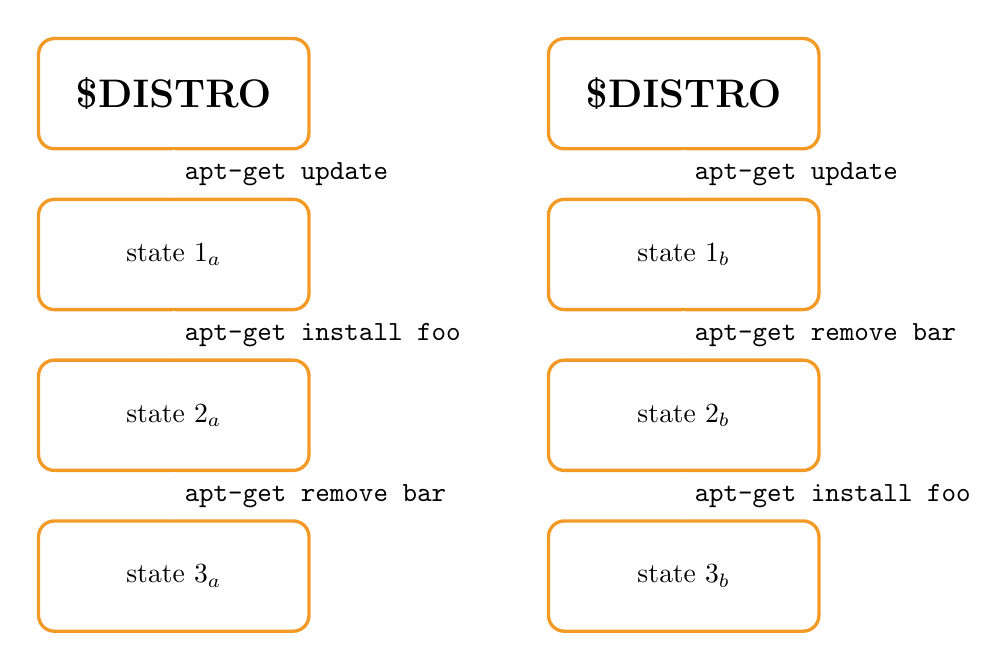
\begin{tikzpicture}[stylish/.style = {
                        draw=guixorange1, very thick,
                        fill=white, text=black, text width=3.2cm,
                        rounded corners=2mm, minimum height=1.4cm,
                        text centered
                      }]
    \matrix[row sep=6mm, column sep=3cm] {
      \node(inita)[stylish]{\textbf{\Large{\$DISTRO}}};
      & \node(initb)[stylish]{\textbf{\Large{\$DISTRO}}};
      \\

      \node<2->(state1a)[stylish]{state $1_a$};
      & \node<2->(state1b)[stylish]{state $1_b$};
      \\

      \node<3->(state2a)[stylish]{state $2_a$};
      & \node<3->(state2b)[stylish]{state $2_b$};
      \\

      \node<4->(state3a)[stylish]{state $3_a$};
      & \node<4->(state3b)[stylish]{state $3_b$};
      \\
    };

    \path[->, very thick, draw=white]<2->
      (inita) edge node[right]{\texttt{apt-get update}} (state1a);
    \path[->, very thick, draw=white]<3->
      (state1a) edge node[right]{\texttt{apt-get install foo}} (state2a);
    \path[->, very thick, draw=white]<4->
      (state2a) edge node[right]{\texttt{apt-get remove bar}} (state3a);
    
    \path[->, very thick, draw=white]<2->
      (initb) edge node[right]{\texttt{apt-get update}} (state1b);
    \path[->, very thick, draw=white]<3->
      (state1b) edge node[right]{\texttt{apt-get remove bar}} (state2b);
    \path[->, very thick, draw=white]<4->
      (state2b) edge node[right]{\texttt{apt-get install foo}} (state3b);

  \end{tikzpicture}
  \end{overlayarea}

  \begin{tikzpicture}[overlay]
    \node<5>[rounded corners=4, text centered,
          fill=guixorange1, text width=3cm,
          inner sep=5mm, opacity=.75, text opacity=1,
          drop shadow={opacity=0.5}] at (5, 4) {
            \textbf{\Huge{= ?}}
          };
  \end{tikzpicture}
\end{frame}

\begin{frame}[plain]
  \Huge{\#3. Entropy keeps increasing.}
\end{frame}

\setbeamercolor{normal text}{bg=white}
\screenshot{images/environment-modules}
\screenshot[width=0.8\paperwidth]{images/package-managers-cropped}
\screenshot{images/npm-curl-pipe-sh-cropped}

\begin{frame}[plain]
  \begin{tikzpicture}[remember picture, overlay]
    \node [at=(current page.center), inner sep=0pt]
          {\includegraphics[height=\paperheight]{images/universal_install_script}};
    \node [at=(current page.north east), anchor=south east, rotate=90,
           text=black, text opacity=1, fill=white, opacity=.6]{
      \url{http://xkcd.com/1654/}
    };
  \end{tikzpicture}
\end{frame}
\setbeamercolor{normal text}{bg=black}


%% \begin{frame}[plain]
%%   \Huge{It's worse, really.}
%% \end{frame}

%% \setbeamercolor*{normal text}{bg=guixdarkgrey,fg=white}
%% \begin{frame}[plain]
%%   \Large{``Let's Package jQuery: A Javascript Packaging Dystopian
%%     Novella'' by Chris Webber}
%%   \\[2.cm]
  
%%   \url{http://dustycloud.org/blog/javascript-packaging-dystopia/}
%% \end{frame}
%% \setbeamercolor*{normal text}{fg=white,bg=black}

\begin{frame}[plain]
  \Huge{\textbf{Giving up?}}
  \\[1.0cm]
  \uncover<2->{\Large{$\rightarrow$ ``app bundles'' (Docker images \& co.)}}
\end{frame}

\setbeamercolor{normal text}{bg=guixred3,fg=white}
\begin{frame}[plain]
  \begin{quotation}
    \noindent
    \LARGE{``Debian and other distributions are going to be \textbf{that
        thing you run docker on}, little more.''}
  \end{quotation}
  \hfill{--- Jos Poortvliet, ownCloud developer}

  \begin{tikzpicture}[overlay]
    \node [at=(current page.south east), anchor=south east]{
      \url{http://lwn.net/Articles/670566/}
    };
  \end{tikzpicture}
\end{frame}

\setbeamercolor{normal text}{bg=white}
\begin{frame}[plain]
  \begin{tikzpicture}[remember picture, overlay]
    \node [at=(current page.center), inner sep=0pt]
          {\includegraphics[height=\paperheight]{images/dockerfile-owncloud-cropped}};

    \node [at=(current page.center), anchor=south west, overlay,
           text=black, text opacity=1, fill=white, opacity=.7, text width=5cm]
          {\LARGE{It's also that thing you run \emph{inside} Docker!}};
  \end{tikzpicture}
\end{frame}


\begin{frame}[plain]
  \begin{tikzpicture}[remember picture, overlay]
    \node [at=(current page.center), inner sep=0pt]
          {\includegraphics[width=\paperwidth]{images/docker-image-layers-cropped}};
    \node [at=(current page.north east), anchor=north east,
           text=black, text opacity=1, fill=white, opacity=.6]{
      \url{https://imagelayers.io/}
    };
  \end{tikzpicture}
\end{frame}

\screenshot{images/frozen-pizza}
\begin{frame}[plain]
  \begin{tikzpicture}[remember picture, overlay]
    \node [at=(current page.center), inner sep=0pt]
          {\includegraphics[height=\paperheight]{images/docker-security}};
    \node [at=(current page.south east), anchor=south east,
           text=black, text opacity=1, fill=white]{
      \small{\url{https://www.banyanops.com/blog/analyzing-docker-hub/}}
    };
    \node [at=(current page.south west), anchor=south west,
           text=black, text opacity=1, fill=white]{
      \small{May 2015}
    };
  \end{tikzpicture}
\end{frame}

\begin{frame}[plain]
  \begin{tikzpicture}[remember picture, overlay]
    \node [at=(current page.center), inner sep=0pt]
          {\includegraphics[width=0.9\paperwidth]{images/singularity-hpc-wire}};
    \node [at=(current page.south east), anchor=south east,
           text=black, text opacity=1, fill=white]{
      \small{\url{https://www.hpcwire.com/2016/10/20/singularity-containers-easing-scientific-computing}}
    };
  \end{tikzpicture}
\end{frame}
\screenshot[height=\paperheight]{images/arstechnica-snappy-goodbye-apt-yum}
\screenshot[height=\paperheight]{images/flatpak}
\setbeamercolor{normal text}{bg=black}

\begin{frame}[plain]{``app bundles'' are headed wrong}
  \Large{
    \begin{itemize}
    \item difficulty to \highlight{compose} software packages
    \item wrong \highlight{abstraction level}: image vs. package
    \item \highlight{hardly reproducible}: we have the bits, not the
      source
    \item makes it hard to \highlight{customize \& experiment}
    \end{itemize}
  }
\end{frame}

\begin{frame}[plain]
  \begin{tikzpicture}[remember picture, overlay]
    \node [at=(current page.center), inner sep=0pt]
          {\includegraphics[height=\paperheight]{images/hope-hero}};
    \node<2> [at=(current page.center), anchor=north, text=black,
           fill=white, opacity=.5, text opacity=1.,
           rounded corners=2mm, inner sep=1cm]{
      \Huge{\textbf{Make packaging great again!}}
    };
  \end{tikzpicture}
\end{frame}


%%%%%%%%%%%%%%%%%%%%%%%%%%%%%%%%%%%%%%%%%%%%%%%%%%%%%%%%%%%%%%%%%%%%%%%%%%%%%%
\setbeamercolor{normal text}{bg=white}
\begin{frame}[plain]
  \begin{tikzpicture}[remember picture, overlay]
    \node [at=(current page.center), inner sep=0pt]
          {\includegraphics[width=0.7\paperwidth]{images/GuixSD-horizontal-print}};
  \end{tikzpicture}
\end{frame}
\setbeamercolor{normal text}{fg=white,bg=black}

\begin{frame}{Guix}
  \LARGE{
    \begin{enumerate}
    \item transactional package manager
    \item software environment manager
    \item APIs \& tools to customize environments
    \item packaging tools
    \end{enumerate}
  }
\end{frame}

\begin{frame}[fragile]

  \begin{semiverbatim}
\$ guix package -i gcc-toolchain coreutils sed grep
\textrm{...}

\$ eval `guix package --search-paths`
\textrm{...}

\$ guix package --manifest=my-software.scm
\textrm{...}
  \end{semiverbatim}

  %% \begin{tikzpicture}[overlay]
  %%   \node[rounded corners=4, text centered,
  %%         fill=guixorange1, text width=3cm,
  %%         inner sep=3mm, rotate=5, opacity=.75, text opacity=1,
  %%         drop shadow={opacity=0.5}] at (5, 4) {
  %%           \textbf{\large{demo}}
  %%         };
  %% \end{tikzpicture}
\end{frame}

\setbeamercolor{normal text}{bg=guixdarkgrey,fg=guixred3}
\begin{frame}[fragile]
  \Huge{Want to get started hacking on hwloc?}
  \\[2cm]
  \uncover<2->{\Large{A simple matter of installing the deps, right?}}
\end{frame}

\setbeamercolor{normal text}{bg=white}
\begin{frame}[plain]
  \begin{tikzpicture}[remember picture, overlay]
    \node [at=(current page.center), inner sep=0pt]
          {\includegraphics[height=\paperheight]{images/hwloc-graph}};
  \end{tikzpicture}
\end{frame}
\setbeamercolor{normal text}{fg=white,bg=black}


\begin{frame}[fragile]
  \begin{semiverbatim}
\$ guix environment --container hwloc
\textrm{...}

\$ guix environment --container hwloc \\
     --ad-hoc git autoconf automake gdb
\textrm{...}

  \end{semiverbatim}
\end{frame}

\begin{frame}[fragile]
  %% \frametitle{Bit-Reproducible Builds$^*$}
  %% \framesubtitle{$^*$ almost!}

  \begin{semiverbatim}
\$ guix build hello
\uncover<2->{/gnu/store/\tikz[baseline]{\node[anchor=base](nixhash){\alert<2>{h2g4sf72\textrm{...}}};}-hwloc-1.11.2}

\uncover<3->{\$ \alert<3>{guix gc --references /gnu/store/\textrm{...}-hwloc-1.11.2}
/gnu/store/\textrm{...}-glibc-2.24
/gnu/store/\textrm{...}-gcc-4.9.3-lib
/gnu/store/\textrm{...}-hwloc-1.11.2
}
  \end{semiverbatim}

  \begin{tikzpicture}[overlay]
    \node<1>(labelnixhash) [fill=white, text=black] at (current page.center) {%
      \Large{\textbf{isolated build}: chroot, separate name spaces, etc.}
    };

    \node<2>(labelnixhash) [fill=white, text=black] at (4cm, 2cm) {%
      hash of \textbf{all} the dependencies};
    \path[->]<2>(labelnixhash.north) edge [bend left, in=180, out=-45] (nixhash.south);

    \draw<4-> (-10pt, 105pt) [very thick, color=guixorange2, rounded corners=8pt]
      arc (10:-50:-50pt and 110pt);
    \node<4->[fill=white, text=black, text opacity=1, opacity=.7,
          rounded corners=2mm, inner sep=5mm]
      at (7, 2) {\textbf{\Large{(nearly) bit-identical for everyone}}};
    %% \node<5>[fill=white, text=black, text opacity=1, opacity=.7,
    %%       rounded corners=1mm, inner sep=3mm]
    %%   at (8, 1) {\url{http://reproducible.debian.net}};
  \end{tikzpicture}

\end{frame}

\setbeamercolor{normal text}{bg=guixdarkgrey,fg=guixred3}
\begin{frame}[plain]
  \Huge{Can we go\\
    \textbf{beyond mere reproducibility}
    \\and support \textbf{experimentation}?}
\end{frame}
\setbeamercolor{normal text}{fg=white,bg=black}

\setbeamercolor{normal text}{bg=white}
\begin{frame}[plain]
  \begin{tikzpicture}[remember picture, overlay]
    \node [at=(current page.center), inner sep=0pt]
          {\includegraphics[height=0.9\paperheight]{images/reppar-front-page}};
    \node [at=(current page.south east), anchor=south east,
           text=black, text opacity=1, fill=white, opacity=.6]{
      \url{https://hal.inria.fr/hal-01161771/en}
    };
  \end{tikzpicture}
\end{frame}
\setbeamercolor{normal text}{fg=white,bg=black}

\begin{frame}[plain]
  \Huge{Creating package variants at the command line}
\end{frame}

\begin{frame}[fragile]
  \begin{semiverbatim}
\$ guix build hwloc \\
    \alert<1>{--with-source}=./hwloc-42.0rc1.tar.gz
\textrm{...}

\pause
\$ guix package -i mumps \\
     \alert<2>{--with-input}=scotch=pt-scotch
\textrm{...}

  \end{semiverbatim}
\end{frame}

\begin{frame}[plain]
  \Huge{Your personal packages or variants in
    \texttt{GUIX\_PACKAGE\_PATH}!}
\end{frame}

%% \begin{frame}[plain]
%%   \Huge{Security updates ``grafted'' onto available binaries}
%% \end{frame}

%% \screenshot{images/hwloc-graph}

\begin{frame}[plain]
  \begin{tikzpicture}[remember picture, overlay]
    \node [at=(current page.center), inner sep=0pt]
          {\includegraphics[width=\paperwidth]{images/os-declaration}};
    \node [at=(current page.center), fill=black, opacity=.3, text
      opacity=1., minimum height=21cm, minimum width=297mm]
          {\huge{\textbf{GuixSD: declarative OS config}}};
  \end{tikzpicture}
\end{frame}

\setbeamercolor{normal text}{bg=guixblue2}
\begin{frame}[plain]
  \Huge{\textbf{Status.}}
\end{frame}
\setbeamercolor{normal text}{fg=white,bg=black}

\begin{frame}
  \Large{
  \begin{itemize}
    \item started in 2012
    \item \highlight{4,400+ packages}, all free software
    \item \highlight{4 architectures}:\\
      x86\_64, i686, ARMv7, mips64el
    \item binaries at \url{https://hydra.gnu.org}
    \item 0.11.0 released in August 2016
  \end{itemize}
  }
\end{frame}

\begin{frame}{cluster deployments \& usage}
  \Large{
    \begin{itemize}
    \item \highlight{Max Delbrück Center} (DE): 250-node cluster +
      workstations
      % https://ubc.uu.nl/infrastructure/
      % https://wiki.bioinformatics.umcutrecht.nl/pub/HPC/WebHome/HPC_Flyer.png
    \item \highlight{Utrecht Bioinformatics Center} (NL): 68-node
      cluster (1,000+ cores)
    \item \highlight{GeneNetwork}, ``framework for web-based genetics''
    \end{itemize}
  }
\end{frame}

\setbeamercolor{normal text}{bg=white}
\screenshot[height=.9\paperheight]{images/openhub-activity}
\screenshot[height=.9\paperheight]{images/openhub-contributors}
\setbeamercolor{normal text}{bg=black}

\setbeamercolor{normal text}{bg=guixblue2}
\begin{frame}[plain]
  \Huge{\textbf{Wrap-up.}}
\end{frame}
\setbeamercolor{normal text}{fg=white,bg=black}

\begin{frame}{Summary}
  \Large{
    \begin{itemize}
    \item Guix supports \highlight{reproducible software environments}
    \item ... can be extended with \highlight{personal packages}
    \item ... allows for \highlight{experimentation} through customization
    \item ... is entirely \highlight{programmable}
    \end{itemize}
  }
\end{frame}

%%%%%%%%%%%%%%%%%%%%%%%%%%%%%%%%%%%%%%%%%%%%%%%%%%%%%%%%%%%%%%%%%%%%%%%%%%%%%%
\begin{frame}[plain]

\vfill{
  \vspace{2.5cm}
  \center{\includegraphics[width=0.2\textwidth]{images/GuixSD}}\\[1.0cm]
  \texttt{ludo@gnu.org}\hfill{\alert{\url{https://gnu.org/software/guix/}}}
}

\end{frame}

\begin{frame}{}

  \begin{textblock}{12}(2, 8)
    \tiny{
      Copyright \copyright{} 2010, 2012--2016 Ludovic Courtès \texttt{ludo@gnu.org}.\\[3.0mm]
      GNU GuixSD logo, CC-BY-SA 4.0, \url{http://gnu.org/s/guix/graphics}

      Copyright of other images included in this document is held by
      their respective owners.
      \\[3.0mm]
      This work is licensed under the \alert{Creative Commons
        Attribution-Share Alike 3.0} License.  To view a copy of this
      license, visit
      \url{http://creativecommons.org/licenses/by-sa/3.0/} or send a
      letter to Creative Commons, 171 Second Street, Suite 300, San
      Francisco, California, 94105, USA.
      \\[2.0mm]
      At your option, you may instead copy, distribute and/or modify
      this document under the terms of the \alert{GNU Free Documentation
        License, Version 1.3 or any later version} published by the Free
      Software Foundation; with no Invariant Sections, no Front-Cover
      Texts, and no Back-Cover Texts.  A copy of the license is
      available at \url{http://www.gnu.org/licenses/gfdl.html}.
      \\[2.0mm]
      % Give a link to the 'Transparent Copy', as per Section 3 of the GFDL.
      The source of this document is available from
      \url{http://git.sv.gnu.org/cgit/guix/maintenance.git}.
    }
  \end{textblock}
\end{frame}

\end{document}

% Local Variables:
% coding: utf-8
% comment-start: "%"
% comment-end: ""
% ispell-local-dictionary: "american"
% compile-command: "rubber --pdf talk.tex"
% End:

%%  LocalWords:  Reproducibility
